\documentclass[
    border={
        3mm % left
        3mm % bottom
        3mm % right
        3mm % top
        }
    ]{standalone}

\usepackage{pagecolor}
\usepackage{tikz}

\definecolor{white}{HTML}{eceff4}

\begin{document}

\pagecolor{white}

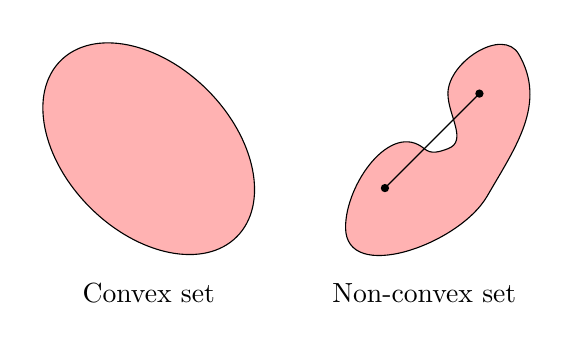
\begin{tikzpicture}
    \begin{scope}
        \draw[rotate=-45,fill=red!30] (0,0) ellipse (45pt and 30pt);
        \node [label={[yshift=-2.2cm]Convex set}] {};
    \end{scope}
    \begin{scope}[xshift=3.5cm]
        \useasboundingbox (-1,-1.35) rectangle (1.5,1.35);
        \draw[fill=red!30] (0,0) to [out=140,in=90] (-1,-1)
        to [out=-90,in=240] (0.8,-0.6)
        to [out=60,in=-60] (1.2,1.2)
        to [out=120,in=90] (0.3,0.7)
        to [out=-90,in=20] (0.3,0)
        to [out=200,in=-40] (0,0);
        \draw (-0.5,-0.5) -- (0.7,0.7);
        \fill (-0.5,-0.5) circle[radius=1.5pt];
        \fill (0.7,0.7) circle[radius=1.5pt];
        \node [label={[yshift=-2.2cm]Non-convex set}] {};
    \end{scope}
\end{tikzpicture}

\end{document}